\newpage

\section{Sumador Inversor}
\begin{figure}[htb]
	\centering
	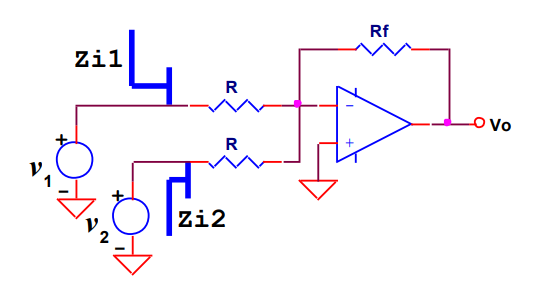
\includegraphics[width=1\textwidth]{figuras/lab_2_circuito.png}
	\caption{Circuito propuesto}
\end{figure}

\subsection{Requisitos}
Para el desarrollo del presente trabajo se empleará un circuito sumador inversor utilizando el amplificador operacional \textit{LM324}. El circuito debe cumplir con las siguientes especificaciones:
\begin{itemize}
    \item $V_{cc}=10[V]$ y $V_{ss}=-10[V]$
    \item $A_{v|v_1}=30$, $A_{v|v_2}=30$
    \item $R_i<<Z_{i1}$, $R_i<<Z_{i2}$
    \item Emplear resistencias menores a $10[M\Omega]$
\end{itemize}

\newpage

\section{Análisis teórico}
A continuación se obtienen las ecuaciones pertinentes para el cálculo de errores.

\subsection{Ganancia ideal en banda de paso}
\onehalfspacing
\begin{flushleft}
    \textbf{Pasivando $V_2$}\\
    $V_{O}|_{V_2=0}=-\frac{R_f}{R}$ \\
    \textbf{Pasivando $V_{1}$} \\
    $V_{O}|_{V_{1}=0}=-\frac{R_f}{R}$ \\
\end{flushleft}
\begin{center}
    \boxed{V_{O}=A_1\cdot v_1 + A_2 \cdot v_2}\\
    reemplazando con $A_1=A_2=-\frac{R_f}{R}$ \\
    \boxed{V_{O}=-\frac{R_f}{R}\cdot (v_1+v_2)}
\end{center}

\subsection{Errores en DC}
\onehalfspacing
Del circuito general, pasivando las entradas, se calcula la ganancia de lazo.
\begin{center}
    \boxed{T(S)=-\frac{R}{R+2R_f}\cdot A_d(S)}
\end{center}
Para obtener las ecuaciones que describen cada error se emplea la ecuación de $Blackman$ y se suponen el resto de las característiscas del amplificador ideal a excepción de la de interés.

\subsubsection{Error por tensión de offset, $v_{os}$}
\onehalfspacing
El error por tensión de offset se estima colocando en la entrada no inversora una fuente de tensión constinua de valor $v_{os}$
\begin{center}
    \boxed{\frac{V_{O}}{V_{os}} = 1 + \frac{R_f}{R_p}}\\
    donde $R_p=\frac{R}{2}$; reemplazando \\
    \boxed{V_{O} = (1 + 2\cdot\frac{R_f}{R}) \cdot v_{os}}
\end{center}

\subsubsection{Error por corrientes de bias, $I_{os}$}
\onehalfspacing
Debido a que no hay una resistencia asociada a la entrada no inversora la corriente $I^{+}_p$ no produce error, en consecuencia el error en la salida solo está definido por $I^{-}_p$
\begin{center}
    \boxed{\frac{V_O}{V^{-}}=\frac{R+2R_f}{R}}
\end{center}
Donde $V^{-}=I^{-}_p\cdot R_p$, $R_p=\frac{R_f\cdot R}{2R_f+R}$, por lo que resulta,
\begin{center}
    \boxed{V_O(I_p^{-})=-I_p\cdot R_f}
\end{center}

\subsubsection{Error por $A_d<\infty$}
\onehalfspacing
La ganancia real de un amplificador puede definirse como:
\begin{center}
    \boxed{A_v(s)=\frac{A_{vfi}}{1-\frac{1}{T(s)}}}
\end{center}
Donde:
\begin{itemize}
    \item $A_{vfi}:$ ganancia ideal para la configuración seleccionada.
    \item $T(s):$ ganancia de lazo.
\end{itemize}
\paragraph{}
Si $A_d(s)\rightarrow \infty$ entonces $T(s) \rightarrow \infty$ por lo que el error para $A_d(s)<\infty$ como:
\begin{center}
    \boxed{\epsilon_{G0}=\frac{1}{T_O}}
\end{center}
\paragraph{}
Luego,
\begin{align}
    \nonumber
    A_{vf}(s) &= \frac{A_{vfi}}{1 + \epsilon_G(s)} \\
    \nonumber
    A_{vf}(0) &= \frac{A_{vfi}}{1 + \epsilon_G(0)} \\
    \nonumber
    A_{vf}(0) &= A_{vfi}(1-\epsilon_G(0))
\end{align}
\paragraph{}
Despejando $\epsilon_G(0)$ y reordenando,
\begin{center}
    \boxed{\Delta V_0 = \epsilon_G(0)\cdot V_{0i}}
\end{center}
\paragraph{}
De la ecuación anterior se tiene que el máximo error sucede cuando $V_{0i}=FS$,
\begin{center}
    \boxed{\Delta V_{0, max}(A_d<\infty)=\epsilon_G(0)\cdot FS=\frac{FS}{T_O}}
\end{center}

\subsubsection{Error por $RRMC<\infty$}
\onehalfspacing
Debido a que la entrada no inversora está conectada a masa el error producido por $RRMC<\infty$ resulta despreciable ya que la tensión común es mínima.

\newpage

\subsection{Errores en AC}
\onehalfspacing
Para el análsis en AC se debe contemplar la expresión que define el comportamiento de la ganancia del amplificador en función de la frecuencia.
\begin{center}
    \boxed{A_{vf}(s)=\frac{A_{vf}(0)}{(1+\frac{s}{\omega_H})}}
\end{center}

\subsubsection{Ancho de banda a plena potencia}
\onehalfspacing
Se define como la máxima frecuencia que puede presentar la señal de entrada para ser reproducida en la salida sin distorsión,
\begin{center}
    \boxed{\omega_{HP}=\frac{SR}{V_{pp}}}
\end{center}
de donde,
\begin{itemize}
    \item $SR:$ Slew-Rate.
    \item $V_{pp}:$ Tensión pico a pico máxima.
\end{itemize}

\subsubsection{Ancho de banda de pequeña señal}
\onehalfspacing
Se define así al punto donde la ganancia cae $-3dB$ respesto al valor en la banda de paso. Del producto $GBW$ se obtiene,
\begin{equation}
   \nonumber
   \omega_H \cdot A_{vf} = \omega_T 
\end{equation}
\begin{center}
    \boxed{\omega_H = \frac{\omega_T}{A_{vf}}}
\end{center}

\subsubsection{Error vectorial}
\onehalfspacing
Se define como la diferencia entre la ganancia ideal y la real:
\begin{center}
    \boxed{E_v=A_{vfi}-A_{vf}(s)}
\end{center}
Dado que le resultado lo conforma un vector se puede dividir en \textit{error de ganancia} y \textit{error de fase}.
\paragraph{}
\textbf{Error de ganancia}
\onehalfspacing
Se define de esta manera a la diferencia entre los módulos real e ideal. Normalizando la ecuación para el error vectorial en función de $A_{vfi}$:
\begin{align}
    \nonumber
    e_v&=|1| - \abs{\frac{1}{1+\frac{s}{\omega_H}}} \\
    \nonumber
    e_v &= 1 - \frac{1}{\sqrt{1+\frac{\omega}{\omega_H}^2}}
\end{align}
Se puede proximar a:
\begin{center}
    \boxed{e_v = 1 - \sqrt{1+\frac{\omega}{\omega_H}^2}}
\end{center}

\paragraph{}
\textbf{Error de fase}
\onehalfspacing
Se define como la diferencia entre las fases de la ganancia ideal y la ganancia real:
\begin{center}
    \boxed{\Phi_v = -\arctan{(\frac{\omega}{\omega_H})}+\frac{\pi}{2}}
\end{center}

